\subsection{Реализация алгоритма трилатерации, основанном на пересечении сфер}

С точки зрения геометрии проблема трилатерации - проблема нахождения точки пересечения трех сфер в пространстве. Для того, чтобы эту точку найти, необходимо решить систему уравнений. Обычно для упрощения промежуточных вычислений полагается, что центры этих сфер лежат на плоскости, определяемой уравнением $z=0$. Кроме того, скажем, что центр первой сферы находится в начале координат, а центр второй лежит на оси $x$. Очевидно, что данная формулировка задачи не уменьшает общности, и задача по сути осталась той же. С другой стороны, к такому виду может быть приведен любой набор из трех сфер. Решив уравнение в преобразованной системе координат, можно вернуться к начальной.

С первого взляда может показаться, что задача определения координаты устройства по нескольким маячкам схожа с задачей, которая решается спутниками GPS, и, соответственно, мы тоже должны решать задачу о пересечении сфер. К тому же, маяки могут быть закреплены в помещении на разных высотах. Но на практике этим можно пренебречь, отбросив $z$-координату. Предпосылкой для этого является и то, что хотя маячки могут находиться на различной высоте, на одной и той же высоте находится пользователь. Таким образом, задача сводится к работе с окружностями.

\begin{figure}
    \centering
    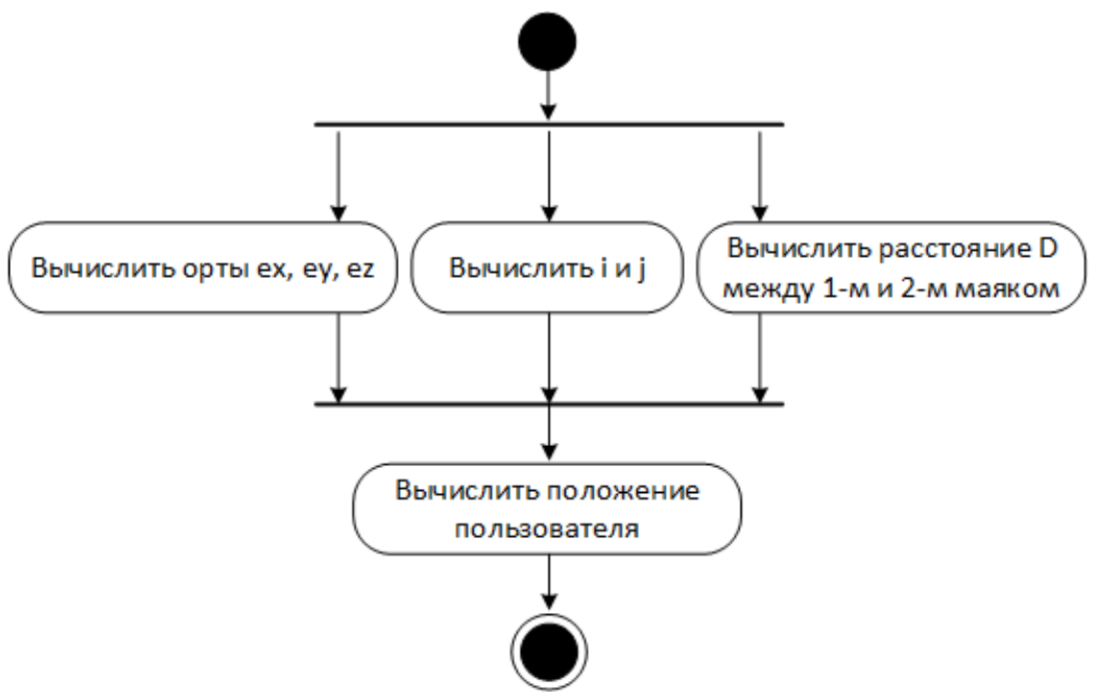
\includegraphics[scale=0.7]{img/sphereIntAct}
    \caption{Диаграмма деятельности алгоритма пересечения сфер}
\end{figure}